% Chapter 2

% Main chapter title
\chapter{Traffic Prediction: Literature Review}

% For referencing the chapter elsewhere, use \ref{Chapter2}
\label{Chapter2}

% This is for the header on each page - perhaps a shortened title
\lhead{Chapter 2. \emph{Traffic Prediction: Literature Review}}

% Quotation
{``There is no way that we can predict the weather six months ahead beyond giving the seasonal
average"}
\begin{flushright}
Stephen Hawking, \textit{Black Holes and Baby Universes} (1993)
\end{flushright}

%---------------------------------------------------------------------------------------------------
%	CONTENT
%---------------------------------------------------------------------------------------------------
\section{Introduction}
In this chapter we provide an account of various elements involved in short term traffic prediciton
as a process and a reasonably complete review of existing literature. Research on short term traffic
prediction has been active since 1979, \citet{ahmed1979analysis}. Yet many professionals around the
world still show a strong interest in this field.
The simplest reseaon being the complex non-linear nature of traffic data and the effects of
non-recurrent events(weather, public events, accidents etc.) on it.  Critical reviews of existing
literature on short term traffic flow have been presented in detail by \citet{smith1997traffic},
\citet{vlahogianni2004short}, \citet{van2012short} and \citet{vlahogianni2014short}. The use of
the phrase 'short term' limits the scope of traffic prediction in terms of the prediction horizon
which usually varies between few seconds to few hours depending upon the approach and application.

The process of short term traffic prediction consists of determining the scope, formulating the
conceptual output specifications and model selection (\citet{vlahogianni2004short}) as shown in
figure \ref{fig:sttp-process}.

\begin{figure}[htbp]
  \centering
    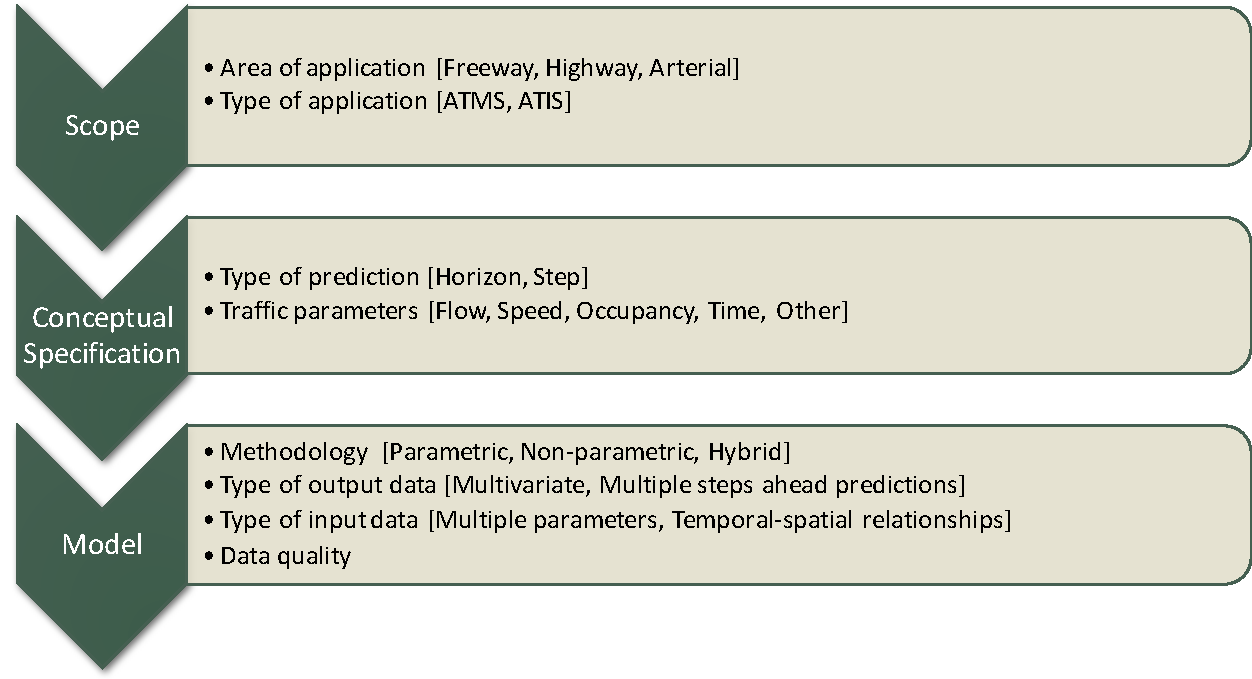
\includegraphics[width=0.7\textwidth,height=0.7\textheight,keepaspectratio]{Figures/sttp-process.pdf}
    \rule{35em}{0.5pt}
  \caption[Elements of short term traffic prediction]{Elements of short term traffic prediction}
  \label{fig:sttp-process}
\end{figure}

Determining whether the prediction model to be developed is going to be part of an advanced
traffic management system or advances traveller information system is important and is influenced
by other elements such as type of road and traffic parameters invloved.

The type of area influences the prediction process. Short term traffic predictions can be done for
highway, freeway and urban arterial roads. Most of the existing work focus on either highway or
freeway traffic. The reason being predcting traffic conditions at a unrban setting is more complex.
While predicting traffic conditions at highways and freeways are important for both advanced traffic
management systems and advances traveller information systems, for urban settings the need for short
term traffic predictions is more relevant for signal control at intersections.

The traffic parameter that are predicted can be - flow(number of vehicles per hour), time(minutes
to travel between two points), speed(mean speed in km/hour) and density(number of vehicles per km).
Relevane of flow is more stable and important than other parameters as per \citet{levin1980forecasting}.
However this is conflicting and other authors have argued otherwise. \citet{dougherty1997short} attempted
to determine the parameter that best describes the traffic conditions and their findings suggested that
flow and density are more relevant than speed. Predicting travel time has also been the focus of many
works, especially in recent years. This is because of its importance when it comes to advances traveller
information systems, while flow and density are more important for advanced traffic management systems.

Selecting the right model for short term traffic prediction is a challenging task. A number of
models have been suggested and yet there is no concensos on a globally acceptable one. The various
methods that have been suggested for short term traffic prediction can be categorised into four
groups - naïve, parametric, non-parametric and hybrid as shown in figure \ref{fig:sttp-methods}.

\begin{figure}[htbp]
  \centering
    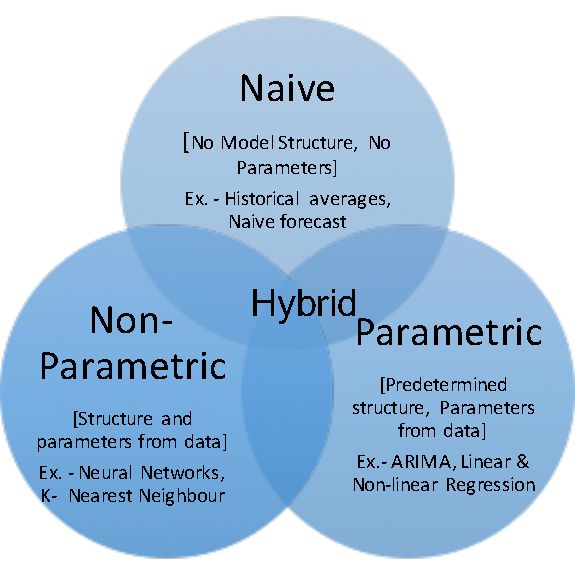
\includegraphics[width=0.4\textwidth,height=0.4\textheight,keepaspectratio]{Figures/sttp-methods.pdf}
    \rule{35em}{0.5pt}
  \caption[Methods in short term traffic prediction]{Methods in short term traffic prediction}
  \label{fig:sttp-methods}
\end{figure}

In the follwing sections, we review significant amount of previous work in this field, grouped by the
type of method.

\section{Naïve methods}
These are heuristics methods, and often used in practice because of their simplicity and the ease
of implementations. In most cases these methods are used as baselines for comparison while
creating more advances methods. We breifly present these methods here.

\subsection{The Naïve method}
The simplest naive approach in short term prediction would be to take the last observed value and
this involves no computational effort. That is at any time t

        \begin{equation}
            \hat{x}_{t} = x_{t-1}
        \end{equation}

Another variant of this method known as seasonal Naïve method, where the estimate at any time t is
last observed value from the same season of the year. This is mainly used for highly seasonal time
series data.

\subsection{Average method}
Another simple heuristic method known as the historical averages uses the average of past observed
values. We define this as

        \begin{equation}
            \hat{x}_{t} = (x_{t-1} + x_{t-2} ... + x_{t-n})/n
        \end{equation}

\section{Parametric methods}
In parametric models, we estimate the parameters from the training dataset to determine the
function that classifies new unseen data. The number of parameters are fixed. The advantage of
parametric models are that these perform quite well in situations where the large amount of data
is not available. Some of the typical examples of parametric models include Linear and
nonlinear regression, ARIMA models, Kalman filter, Linear SVM etc.

\subsection{Classical regression}
In machine learning and statistical applications, the use of linear models are predominant. These
models are also important in time series domains such as traffic flow prediction. The primary
idea behind the regression is to express the output variable as a linear combination of input
vectors. We can express the linear regression in time series as an ouput influenced by a
collection of inputs, where the inputs could possibly be an independent series

        \begin{equation}
            x_{t} = \beta_{1}z_{t1} + \beta_{2}z_{t2} + ... + \beta_{q}z_{tq} + w_{t}
        \end{equation}

where $ \beta_{1}, \beta_{2},...,\beta_{q} $ are unknown regression coeffiecients and $w_{t}$ is
a random error.

A very few attempts have been made to model the traffic conditions using linear and non-linear
models of regression in the field of short term traffic prediction. The simplest reason being the
inability of these statistical methods to capture the highly non-linear and complex relationships that
are present in the traffic data.
\citet{low1972new} and \citet{jensen1973calibrating} used linear models of regresion for predicting
traffic volumes while \citet{hogberg1976estimation} used non-liner regression for traffic prediction.
\citet{lan1999real} proposed a recursive algorithm by using a dynamic genralised linear model
in this context to predict traffic flow. In this work a negative binomial probabilty distribution
was chosen. The flow data used in this experiment was obtained using a video camera and counted
manually and hence very small set of data set containinh 139 observations at 20 seconds interval
was used for model evalution.

\subsection{ARIMA}
ARIMA(Auto Regressive Integrated Moving Average) is a class of parametric regression models. In
this section we will introduce ARIMA and related methods such as exponential smoothing and moving
averages. For an in depth understanding of these models the reader is encouraged to refer to to
~\citet{tong1990non}, ~\citet{brockwell2006introduction} and ~\citet{box2015time}. It is
important to understand that ARIMA modelling works only with stationary time series data. A
stationary time series is one whose properties do not depend on the time it is being observed.
Trends and seasonality affect time series and hence make it non-stationary. Although this seems as a
big restriction, in short term traffic prediction, ARIMA models have been very successful. Two
basic models constituate ARIMA models - AR(autoregressive) and MA(moving average).

The main idea behind autoregressive models is that past values affect the present value, i.e.
$x_{t}$ can be expressed as a function of past p values $ x_{t-1}, x_{t-2},...,x_{t-p} $ , where
p is the number of steps into the past. We can express an autoregressive model of order p as below

        \begin{equation} \label{eq:autoregressive}
          x_{t} = \phi_{1}x_{t-1} + \phi_{2}x_{t-2} + ... + \phi_{p}x_{t-p} + w_{t}
        \end{equation}

where $x_{t}$ is stationary and $\phi_{1}, \phi_{2},..., \phi_{p}$ are constant
parameters that are to be chosen. We have added the term $w_{t}$ as a Guassian white noise with
zero mean and variance $\sigma^{2}_{w}$.

In the MA model, the current value is dependent on the last q one-step forecast errors
$e_{t-1}, e_{t-2},...,e_{t-q}$ and the white noise $w_{t}$. The expression for moving average
is

        \begin{equation} \label{eq:movingaverage}
          x_{t} = -\theta_{1}e_{t-1} - \theta_{2}e_{t-2} - ... - \theta_{q}e_{t-q} + w_{t}
        \end{equation}

$\theta_{1}, \theta_{2},..., \theta_{q}$ are the parameters to be chosen.

Now proceeding to an ARMA(autoregressive moving average) model, we define an ARMA(p,q) model
where the present value $x_{t}$ is dependent on p past recent values and q past recent forecast
errors and a white noise $w_{t}$.

        \begin{equation} \label{eq:arma}
          x_{t} = \phi_{1}x_{t-1} + \phi_{2}x_{t-2} + ... + \phi_{p}x_{t-p} - \theta_{1}e_{t-1}
          - \theta_{2}e_{t-2} - ... - \theta_{q}e_{t-q} + w_{t}
        \end{equation}

When q is 0, the model becomes an autoregressive model of order p, AR(p) and when p is 0 the model
is a moving average of order q, MA(q). We can rewrite \ref{eq:arma} by using the backshift
operator $B^{\alpha}$, which is defined as $B^{\alpha}z_{t} = z_{t-\alpha}$,

        \begin{equation} \label{eq:armarewrite}
          \phi(B)x_{t} = \theta(B)e_{t}
        \end{equation}

where
        \begin{equation}
            \phi(z) = 1 - \phi_{1}z - ... - \phi_{p}z^{p}
        \end{equation}
        \begin{equation}
            \theta(z) = 1 - \theta_{1}z - ... - \theta_{q}z^{q}
        \end{equation}

In practice, most time series data are non-stationary and so several approaches, for instance
by differencing, are taken to make it stationary before applying the ARMA(p,q) model. By
combining differencing with autoregressive and moving average we obtain the ARIMA model defined
as below
        \begin{equation} \label{eq:arima}
          x'_{t} = \phi_{1}x'_{t-1} + \phi_{2}x'_{t-2} + ... + \phi_{p}x'_{t-p} -
          \theta_{1}e_{t-1} - \theta_{2}e_{t-2} - ... - \theta_{q}e_{t-q} + w_{t}
        \end{equation}

where $x'_{t}$ is the differenced series. Formally the model is denotes as ARIMA(p,d,q) where p
is the order of autoregressive part, d is the degree of differencing and q is the order of moving
average. This is also known as a non-seasonal ARIMA model.

The common method used to determine the parameters in an ARIMA(p,d,q) model is known as the
Box-Jenkins approach (\citet{box2015time}) which is three stage procedure. The three stages are
identification, estimation and diagnostic checking. At the identification stage, the values p, d
and q are determined by observing the autocorrelation and partial autocorrelation functions of
the time series and its differences. At the estimation stage, the maximum liklihood estimates are
determined for each model parameter. Finally in the dignostics stage, the residuals are analysed
and model comparisions are done. If the model fits well then the standardised residuals behave as
an i.i.d. with mean zero and variance one.

\citet{ahmed1979analysis} used Box-Jenkins method for short-term traffic forecast. The input data
used was 166 sets of time series traffic data collected by freeway traffic surveillance systems in
three locations - Los Angeles, Minneapolis and Detroit. The authors concluded an ARIMA(0,1,3)
model, based on the autocorrealtion and partial autocorrelation functions, as a resonable fit for
the short term prediction tasks for both traffic volume and occupancy. The model performance was
evaluated against a moving average, a double smoothing average and a Trigg and Leach adaptive
model. The comparisons suggest that the ARIMA model had better accuracy than the others. The
authors used this model in detecting traffic incidents by comparing the real-time flow occupancy
with the predicted value. \citet{nihan1980use} used the Box-Jenkins technique on monthly data
collected at 15 minutes interval on a freeway segment from 1968 to 1976 to forecast for the year
1977. After examining several models they finally selecte an ARIMA(12,1,7) model. The forecast
was done for average weekday volume with positive results. \citet{hamed1995short} studies the
application of ARIMA model in short term traffic volume prediction. They found a simple ARIMA(0,1,1)
model to be adequate for modelling the traffic data. The used a 1-min interval dataset collected in
five urban aretrials.

\citet{williams2001multivariate} used an ARIMAX model to use upstream traffic data along with the
predicting location's traffic data while estimating the paramters of the ARIMA model. This is
done using ARIMAX model which is an extension of the ARIMA model where an exogenous variable is
used. The data was collected form four locations near Beaune, France. The data from three upstream
locations were used for forecasting at the fourth location in Beaune. The same data were used
in the proposed ATHENA and KARIMA models. The model was compared  against the univariate ARIMA,
ATHENA\citet{danech1991athena} and KARIMA(\citet{van1996combining}) models. The results show tha
the ARIMAX model consistently outperformed the ARIMA model. However the complexity of the ARIMAX
model is more than the ARIMA model with as many as twice the parameters to estimate. Also in case
of missing values the ARIMAX model performance degraded more than the ARIMA model.

\citet{min2009short} proposed a dynamic Space Time ARIMA (STARIMA) model for short term traffic
prediction. Their argument for the new proposed model was based on the factor that most of the
existed model failed to take the spatial information of the transporatation system into account.
The proposed dynamic STARIMA model combines STARIMA and Dynamic Turn Ratio Prediction (DTRP)
model. Using DTRP they dynamically updated the static matric $W_{k}$ in STARIMA model that contains
the structural information of the transporatation network. The results of the study showed
significant improvement in forecast accuracy. The authors later published another similar work
(\citet{min2010urban}) that used the generalised STARIMA (GSTARIMA) model.  The authors
presented the results where this model has a small improvements over the STARIMA model. However
the major drawbacks of the GSTARIMA model is the estimation of large number of parameters which
significantly increases the computational time. It also suffers in performance if enough historical
data is not available.

\citet{williams2003modeling} poposed for the acceptance of seasonal ARIMA models for short term
traffic prediction. A seasonal ARIMA $(p,d,q) (P,D,Q)_{s}$ for a time series {$x_{t}$} is one
where s is the period, d and D are nonnegative integers. The time series theorem known as the World
decomposition is used as the theoritical justification of applying seasonal ARIMA model to
univariate time series with stationarity. Data from two freeway locations, one each from the
United States and the United Kingdom were used for evaluating the model. The performance of the
models were compared against three heuristics approaches - historical averages, random walk and
deviation from historical avarages. The results show that for both the locations the seasonal
ARIMA has better performance than the three methods mentioned earlier. However the authors did
not present whether a non-seasonal ARIMA model would have similar performance. The only other
model that was considered for comparison was the KARIMA model, which did not perform as good as
the seasonal ARIMA model. \citet{kumar2015short} also used a seasonal ARIMA in the context of
limited data for short term traffic prediction. They used data collected over three days from an
arterial road in Chennai, India for the study. The model was validated on 24 hours ahead forecast.
Thier resluts were positive when compared with historical avereges and naïve methods. They
argued when availability of large traffic dataset is a constraint seasonal ARIMA method is a
better choice. \citet{szeto2009multivariate} used a hybrid SARIMA model with cell transmission
model for multivariate traffic prediction. The authors reasoned the use of multivariate models
captuered the spatial characteristics of the transporatation network and hence are the natural
and better choice over an univariate model. The model was validated against data collected form
the city center in Dublin, Ireland. The results at two junctions were compared against real
observations and had MAPE of 4.45 and 10.6. The authors however did not provide comparison
against other univariate models or multivariate models which could present the model's relative
performance.

The major defficiency of tha ARIMA models is that they do not take the extremes into
consideration and focus on the means. This is in contrast to the nature of the traffic data.
ARIMA models are also have the inability to perform will with missing data as pointed out by
\citet{smith1997traffic}.


\subsection{Kalman filter}
Kalman filter is a paramteric regression technique usually used in the field of automatic control
systems and signal preocessing. It was proposed by \citet{kalman1960new}. It can be used to model
both stationary and non-stationary time series. We present a brief description of this theory, for
detail understanding the reader should refer to some extensive literature (such as
\citet{harvey1990forecasting}  and \citet{haykin2001kalman}).


The Kalman filter solves the problem of sequential state estimation of a dynamic linear system, where
in such a system the state evolution and the measurements are both linear and Gaussian. Let us consider
a state space model of the form

        \begin{equation} x_{n} = P_{n}x_{n-1} + \tau_{n} \end{equation}
        \begin{equation} y_{n} = Q_{n}y_{n-1} + \upsilon_{n} \end{equation}

where, $x_{n}$ and $y_{n}$ are the state and measurement respoectvely at time step n.
$P_{n}$ is a $N \times N$ state transition matrix and $\tau_{n}$ is a $N \times 1$ Gaussian
random state noise vector with zero mean and covariance matrix $R_{n}$. $Q_{n}$ is a $M \times N$
measurement matrix and $\upsilon_{n}$ is a $M \times 1$ Gaussian random measurement noise vector
with zero mean and covariance matrix $S_{n}$.

In this state-space setting, the two important tasks are - \textit{filtering} and \textit{prediction}.
The filtering problem is to estimate the state $x_{n}$ given the set of measurements
$Y_{n} = y_{1}, y_{2},...,y_{n}$. And the prediction probelm is to predict $x_{n+t}$, that is the
state after t time steps, given the set of measurements $Y_{n}$. The Kalman filter algorithm can be
described using the below equations.

        1. Prediction step

        \begin{equation} m_{n|n-1} = P_{n}m_{n-1|n-1} \end{equation}
        \begin{equation} C_{n|n-1} = P_{n}C_{n-1|n-1}P^{T}_{n} + R_{n} \end{equation}

        2. Update step to estimate $\hat{x}_{n} = m_{n|n}$

        \begin{equation} J_{n} = Q_{n}C_{n|n-1}Q^{T}_{n} + S_{n} \end{equation}
        \begin{equation} K_{n} = C_{n|n-1}Q^{T}_{n}J^{-1}_{n} \end{equation}
        \begin{equation} m_{n|n} = m_{n|n-1} + K_{n}(y_{n} - Q_{n}m_{n|n-1}) \end{equation}
        \begin{equation} C_{n|n} = C_{n|n-1} - K_{n}Q_{n}C_{n|n-1} \end{equation}

where $m_{n|n}$ and $C_{n|n}$ are the Gaussian mean and covariance of state $x_{n}$ at time step n,
in the posterior probability distributed function

        \begin{equation} p(x_{n}|Y_{n}) \equiv \mathcal{N}(x_{n};m_{n|n},C_{n|n}) \end{equation}

The subscript notation $n|n$ denotes the recursive computation of the pdf of the state $x_{n}$ at
step n using the measurements upto time step n.

\begin{figure}[htbp]
  \centering
    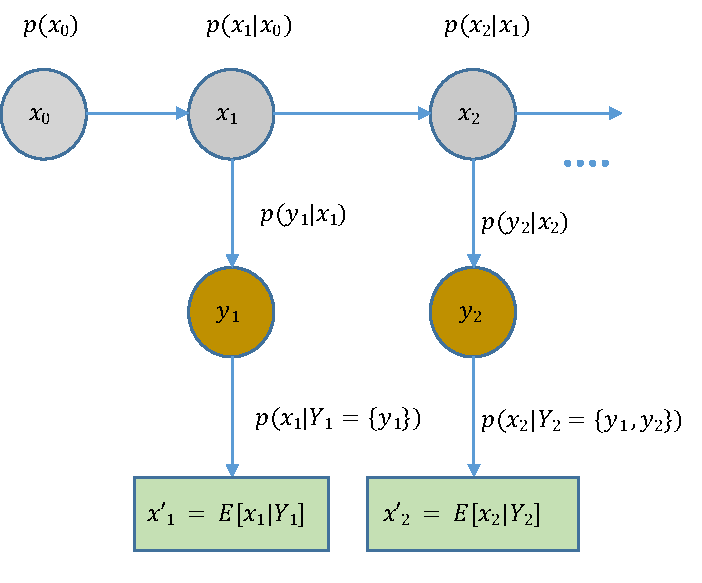
\includegraphics[width=0.5\textwidth,height=0.5\textheight,keepaspectratio]{Figures/kalman-filter.pdf}
    \rule{35em}{0.5pt}
  \caption[Sequential Bayesian estimation in Kalman filtering]{Sequential Bayesian estimation in
  Kalman filtering, recursively computes the posterior probabilty $p(x_{n}|Y_{n})$}
  \label{fig:kalman-filter}
\end{figure}

\citet{okutani1984dynamic} proposed two models using Kalman filtering for short term traffic volume
predictions. The prediction of volume on a link were done using not only the data from that link but
also from adjacent links. They found, using these models, the average error rate to be around 9\%.
This shows the ability of Kalman filtering to predict in a multivariate setting which is difficult in
other statistical regression models such as ARIMA.
\citet{stathopoulos2003multivariate}
\citet{xie2007short} \citet{guo2010real}
\citet{guo2014adaptive}

\section{Non-Parametric methods}
In nonparamtric models the parameters are not fixed, and vary with the amount of data available.
Usually more data is required for this models than parametric models. The advantage of these models
is that they can model the complex non-linear data better. Some of the widely used non-parametric
models are - k-Nearest Neighbour, Support Vector Machines and Neural Networks

\subsection{K-nearest neighbour}
\citet{smith1994comparison} performed a comparison between non-parametric regression and neural
networks. They used a backpropagation neural network model with one hidden layer and k-nearest
neighbour with k value of 10. They showed using their results that nearest neighbour to be more
effective than the neural network model. They also argued their use because nearest neighbour methods
are simple to understand by practitioners.
\citet{lv2009real}

\citet{myung2011travel}

\citet{zhang2013improved}

\citet{meng2015two}


\subsection{Neural networks}
\label{subsec:neuralNetworksTrafficPred}
Artificial Neural Networks(ANN) were mathematical models (\citet{mcculloch1943logical},
\citet{rosenblatt1958perceptron}) designed to  provide a representation of how the human brain
works. It is obvious now that these mathematical models bear little resemblance to the structure
of brain, yet they have been hugely successful. Because they were initially inspired by the
biological brain, the term neural is associated with such kind of mathematical models. A basic
artificial neural network consists of a set of nodes connnected by edges with weights. We can say
that the nodes represent the biological neurons and the edges represent the synapses. The
conections among the nodes can be cyclic or acyclic. The former is known as a feedforward neural
network and the later as a recurrent network. We describe about these neural networks in more
details in chpater \ref{Chapter4}. Several variations of artificial neural networks have been
used in short term traffic prediction. Some well known examples include - \textit{Multilayer
perceptrons, Radial basis function networks, Kohnen maps} and \textit{Hopfield networks}.

\citet{clark1993use} made a comparison of of neural networks and ARIMA models in an urban setting
and found slight difference between the performances. \citet{dougherty1997short} applied a
backpropagation feedforward neural network in traffic flow and speed predictions. They used this
model to predict flow, occupancy and speed traffic parameters and found the prediction of speed to
be disappointing. For flow and occupancy, even though the results were not outstanding, were promising.
\citet{kirby1997should} extended the work of \citet{clark1993use} and compared a neural network model
with the ATHENA and ARIMA models. They concluded that the neural networks performed worse than the
ARIMA model for 30 and 60 minutes prediction horizons. However they argued that the neural networks
are by nature the most suited models to fit the traffic characteristics than the statistical time
series methods. \citet{yasdi1999prediction} used a Jordan neural network for traffic volume predicions.
The authors made forecasts for weekly, daily and hourly traffic volumes. For their work they used
data collected from traffic loop inducters and aggregated at fifteen minutes interval. The data is
then further classified based on events and stored in a knowledge base for reference. The results were
exceptonal with an MSE less than 0.003. \citet{dia2001object} used a time-lag recurrent network(TLRN)
to predict traffic speed for fifteen minutes horizon. They performed their experiment on a section
of the Pacific Highway between Brisbane and Goldcost in Queensland, Australia. Unlike previous mentioned
studies the authors used an object-oriented dynamic neural network model. The dataset they used consisted
of 5000 obsservations at 20 seconds of interval collected over five hour period on two days. Their results
show that the model had an accuracy of 90-94\% for 5 minutes predictions. The accuracies dropped
to 84\% and 80\% for 10 and 15 minutes prediction horizons respectively.
\citet{chen2001use} applied a dynamic neural network model in this context, which was based on a
resource allocating network(RAN). The RAN is a single hidden layer neural network with no inital hidden
units. The hidden units are added dynamically and the number of hidden units correspond to the compexity
of the mapped function. Upto a macimum number of hidden units were set to 30 in this study.
\citet{innamaa2005short}applied a feedforward MLP to predict travel time in an interurban highway.
They used data collected over a period of four months in a highway in southern Finland. The neural
network implemented for the experiment was very simple with one hidden layer and at most 20 units in
the hidden layer. Also they used separate neural networks for each sublink to predict the average
travel time, thus in practice these are unrealistic to be implemented due to increased complexity.
On an average they achieved an accuracy of 90\%. They suggested inclusion of flow information could
have been beneficial. \citet{jiang2005dynamic} used a nonparametric dynamic time-delay recurrent
wavelet neural network model for forecasting traffic flow. They suggested that this model can be
used for both the short term and long term(from a day to a month) traffic flow forecasting. They
used a limited dataset and showed the results to be within 10\% error rate.


Neural networks are very powerful not only in thier good predictive ability but also they are robust
and model the traffic conditions with good overall performance.

\subsection{Support vector machine}

\subsection{Fuzzy logic}

\citet{zhang2008short}

\subsection{Bayesian networks}

\citet{castillo2008predicting}


\section{Hybrid Methods}
In recent years many hybrid methods have been tried in short term traffic prediction with mixed
results.

The ATHENA model(\citet{danech1991athena}) is a hybrid model that employed a layered statistical
approach. It used a clustering method to group the data and then a linear regression model was applied
to each cluster. A hybrid method by combining kohonen maps with ARIMA model was proposed by
\citet{van1996combining}. The model known as KARIMA, used the same data (collected near Beaune,
France) that was used in the ATHENA model for an accurate comparison with the later. The authors
used rectangular and hexagonal Kohonen maps to cluster the traffic volume data. Then each of the
new data cluster was fitted using an ARIMA model. This layered approach was similar to the ATHENA
model. The authors observed the superiority of the hexagonal Kohonen maps over the rectangular one,
but unable to determine the reason of that. Overall the model showed improved performance than the
ATHENA and a simple ARIMA model.

\citet{chen2001study} analysed the use of hybrid neural networks in the context of traffic prediction
and the effect of missing data on those. The authors used two hybrid methods usign the self-organising
maps(SOM). In the first method they used four ARIMA models while in the second method two multi-layer
perceptrons(MLP) were used. The SOM was used to classify the traffic data into different cluster that
can then be used by a suitable ARIMA or MLP model. The SOM/ARIMA performed better than individual
ARIMA models while the SOM/MLP method outperformed all other methods used in the study. They also
observed that the ARIMA models were also the most sensitive to missing data, while neural networks
were mostly unaffected.

\citet{yin2002urban} used a hybrid fuzzy-neural model(FNM) for this task. The FNM model consisted of
two modules - a gate network (GN) and an expert network (EN). The role of the GN is to classify the
input traffic data into a group of clusters using a fuzzy method. On the other hand the EN was a
neural network that models the the clustered data for predictions. An online rolling training scheme
was proposed to train the FNM model. The performance of this model was done with a very simple neural
network model. It was observed clustering the input data beforehand helped improving the overall
performance. It would have been worth comparing the model performance with other hybrid models such
as the KARIMA model that takes a similar approach.

\cite{abdulhai2002short} validated the used of neuro-genetic algorithms in short term traffic flow and
occupancy predictions on a freeway. They used a time delayed neural network (TDNN) model, whose
structure was synthesised by using a genetic algorithm. The model used tried to capture the
tempo-spatial relationships in the traffic conditions by using the traffic data from upstream and
downstream sections. A genetic algorithm was used to chose the neural network from a population. The
model performance was validated using both simulated and real traffic data. The comparisons were made
against a backpropagation feedforward MLP. The model performed acceptably with an accuracy of 86\% for
15 minutes predictions. The model performance was significantly affected for less spatial effects.

\citet{ishak2004optimizing} used a neuro-fuzzy hybrid model.

\citet{vlahogianni2005optimized} used a combined genetic and neural network approach.

\citet{chen2011short} proposed an ARIMA-GARCH model for short term traffic prediction. The
performance of this hybrid model when compared to the standard ARIMA model did not yield positive
results.


\section{Comparisons}
A vast majority of the previous work present some form of comparison between different methods based
on the empirical results. But as the results apply only to a specific area, we can not make these
as the basis for a general comparison between these methods. \citet{smith2002comparison} performed
a comparison between non-parametric and parametric models for single point traffic flow
forecasting based on their theoritical foundations. They found the parameter estimation and outlier
detection using a sesonal ARIMA model is time consuming, hence in practical situations they may not be the
best suited. While ARIMA models have thier foundations in stoachstic system theory, the non-parametric
regression is founded on chaotic system theory. The argument that is in favour of using ARIMA models
is that traffic conditions data are stochastic in nature. Although this is a valid assumption, the
presense of chaotic nature in traffic data can not be dismissed, especially in a congested traffic
environment. \citet{hu2003applicable} explored this and applied phase space reconstruction theory to
forecast traffic flow and found some positive results.

We present a summury of the comparisons among the above mentioned mehods in the table
\ref{table:comparisonExistingMethods}. The comparisons show their overall advantages and disadvantages.

\begin{table}
    \begin{tabular}{c}
        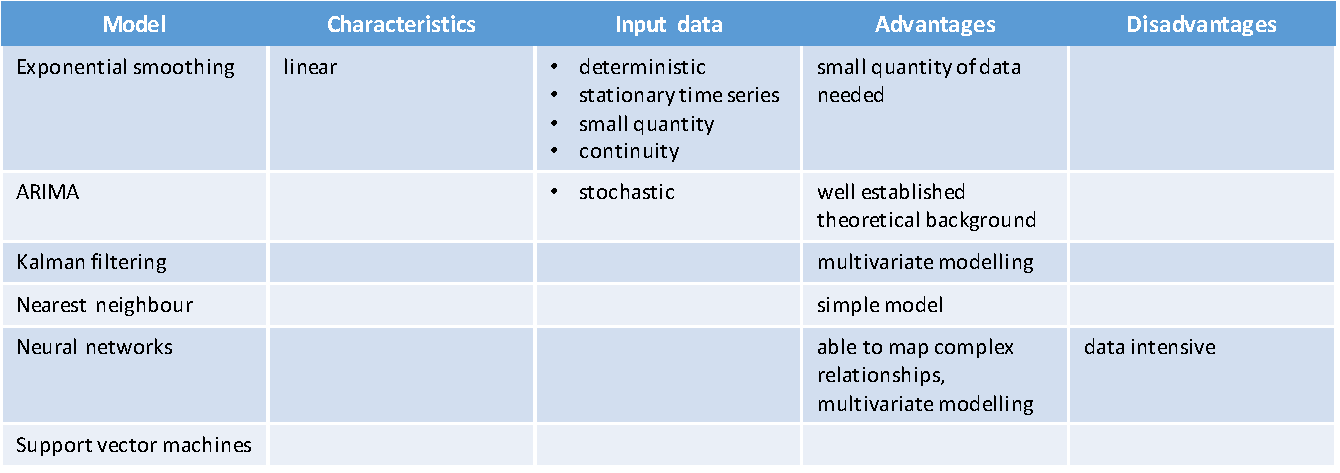
\includegraphics[width=\textwidth,height=\textheight,keepaspectratio]{Figures/method-comparisons.pdf}
    \end{tabular}
    \caption[Comparison of existing methods]{Comparison of existing methods applied in short term
     traffic predictions.}
    \label{table:comparisonExistingMethods}
\end{table}